\documentclass[conference,letterpaper]{IEEEtran}
\IEEEoverridecommandlockouts
\usepackage{cite}
\usepackage{amsmath,amssymb}
\usepackage{graphicx}
\usepackage{booktabs}
\usepackage{array}
\usepackage{xcolor}
\usepackage{url}
\usepackage[hidelinks]{hyperref}

% Every result below is a macro generated from the evaluation outputs
% (make_numbers.py -> numbers.tex for CHB-MIT, make_numbers_s2.py -> numbers_s2.tex for SeizeIT2).
% AUTO-GENERATED by make_numbers.py — do not edit by hand
% source: ../final2
\newcommand{\Pilot}{0}
\newcommand{\PilotNote}{}
\newcommand{\PrimaryCh}{FP1-FP2}
\newcommand{\NPat}{24}
\newcommand{\NRec}{160}
\newcommand{\NSz}{194}
\newcommand{\NHours}{220}
\newcommand{\NSzAll}{198}
\newcommand{\NHoursAll}{225}
\newcommand{\PyBSens}{5.7\%}
\newcommand{\PyBDet}{11}
\newcommand{\PyBCI}{2--11\%}
\newcommand{\PyBFAh}{0.32}
\newcommand{\PyBFAday}{7.7}
\newcommand{\PyBFACI}{0.21--0.47}
\newcommand{\PyBLat}{26.3}
\newcommand{\PyBChance}{1.3\%}
\newcommand{\PyASens}{21.1\%}
\newcommand{\PyADet}{41}
\newcommand{\PyACI}{14--30\%}
\newcommand{\PyAFAh}{2.82}
\newcommand{\PyAFAday}{67.7}
\newcommand{\PyAFACI}{1.99--3.80}
\newcommand{\PyALat}{28.4}
\newcommand{\PyAChance}{10.9\%}
\newcommand{\FwBSens}{75.3\%}
\newcommand{\FwBDet}{146}
\newcommand{\FwBCI}{61--94\%}
\newcommand{\FwBFAh}{18.29}
\newcommand{\FwBFAday}{438.9}
\newcommand{\FwBFACI}{15.23--21.18}
\newcommand{\FwBLat}{14.5}
\newcommand{\FwBChance}{51.5\%}
\newcommand{\FwASens}{85.1\%}
\newcommand{\FwADet}{165}
\newcommand{\FwACI}{79--95\%}
\newcommand{\FwAFAh}{24.98}
\newcommand{\FwAFAday}{599.5}
\newcommand{\FwAFACI}{22.26--27.53}
\newcommand{\FwALat}{14.7}
\newcommand{\FwAChance}{62.4\%}
\newcommand{\LlASens}{27.3\%}
\newcommand{\LlADet}{53}
\newcommand{\LlACI}{15--44\%}
\newcommand{\LlAFAh}{0.98}
\newcommand{\LlAFAday}{23.6}
\newcommand{\LlAFACI}{0.66--1.27}
\newcommand{\LlALat}{20.0}
\newcommand{\LlAChance}{4.0\%}
\newcommand{\LlBSens}{24.2\%}
\newcommand{\LlBDet}{47}
\newcommand{\LlBCI}{13--42\%}
\newcommand{\LlBFAh}{0.47}
\newcommand{\LlBFAday}{11.2}
\newcommand{\LlBFACI}{0.29--0.61}
\newcommand{\LlBLat}{25.0}
\newcommand{\LlBChance}{1.9\%}
\newcommand{\LlCSens}{19.1\%}
\newcommand{\LlCDet}{37}
\newcommand{\LlCCI}{9--34\%}
\newcommand{\LlCFAh}{0.25}
\newcommand{\LlCFAday}{6.0}
\newcommand{\LlCFACI}{0.13--0.38}
\newcommand{\LlCLat}{27.0}
\newcommand{\LlCChance}{1.0\%}
\newcommand{\DevASens}{47.4\%}
\newcommand{\DevADet}{92}
\newcommand{\DevACI}{30--71\%}
\newcommand{\DevAFAh}{0.87}
\newcommand{\DevAFAday}{20.8}
\newcommand{\DevAFACI}{0.60--1.22}
\newcommand{\DevALat}{18.0}
\newcommand{\DevAChance}{3.5\%}
\newcommand{\DevBSens}{41.8\%}
\newcommand{\DevBDet}{81}
\newcommand{\DevBCI}{25--65\%}
\newcommand{\DevBFAh}{0.40}
\newcommand{\DevBFAday}{9.7}
\newcommand{\DevBFACI}{0.25--0.62}
\newcommand{\DevBLat}{23.0}
\newcommand{\DevBChance}{1.7\%}
\newcommand{\DevCSens}{30.4\%}
\newcommand{\DevCDet}{59}
\newcommand{\DevCCI}{16--53\%}
\newcommand{\DevCFAh}{0.18}
\newcommand{\DevCFAday}{4.4}
\newcommand{\DevCFACI}{0.08--0.32}
\newcommand{\DevCLat}{25.0}
\newcommand{\DevCChance}{0.7\%}
\newcommand{\FuASens}{37.1\%}
\newcommand{\FuADet}{72}
\newcommand{\FuACI}{23--58\%}
\newcommand{\FuAFAh}{0.81}
\newcommand{\FuAFAday}{19.5}
\newcommand{\FuAFACI}{0.55--1.09}
\newcommand{\FuALat}{23.5}
\newcommand{\FuAChance}{3.3\%}
\newcommand{\FuBSens}{28.9\%}
\newcommand{\FuBDet}{56}
\newcommand{\FuBCI}{15--50\%}
\newcommand{\FuBFAh}{0.29}
\newcommand{\FuBFAday}{7.1}
\newcommand{\FuBFACI}{0.16--0.46}
\newcommand{\FuBLat}{26.0}
\newcommand{\FuBChance}{1.2\%}
\newcommand{\FuCSens}{29.9\%}
\newcommand{\FuCDet}{58}
\newcommand{\FuCCI}{16--51\%}
\newcommand{\FuCFAh}{0.23}
\newcommand{\FuCFAday}{5.6}
\newcommand{\FuCFACI}{0.13--0.38}
\newcommand{\FuCLat}{27.0}
\newcommand{\FuCChance}{1.0\%}
\newcommand{\DevAParams}{$r{=}1.5$, $D{=}15$\,s; $r{=}1.5$, $D{=}15$\,s}
\newcommand{\DevBParams}{$r{=}1.5$, $D{=}20$\,s; $r{=}1.5$, $D{=}20$\,s}
\newcommand{\DevCParams}{$r{=}2.0$, $D{=}20$\,s; $r{=}2.5$, $D{=}15$\,s}
\newcommand{\TestDevPyP}{$p{=}6{\times}10^{-5}$}
\newcommand{\TestDevPyBetter}{21}
\newcommand{\TestDevPyWorse}{0}
\newcommand{\TestDevPyN}{24}
\newcommand{\TestDevPyAnyP}{$p{=}2{\times}10^{-4}$}
\newcommand{\TestDevPyAnyBetter}{18}
\newcommand{\TestDevPyAnyWorse}{2}
\newcommand{\TestDevPyAnyN}{24}
\newcommand{\TestDevLlP}{$p{=}7{\times}10^{-4}$}
\newcommand{\TestDevLlBetter}{15}
\newcommand{\TestDevLlWorse}{0}
\newcommand{\TestDevLlN}{24}
\newcommand{\FoldDevPy}{7}
\newcommand{\AucLL}{0.70}
\newcommand{\AucLLCase}{0.79}
\newcommand{\MedLLIctal}{108}
\newcommand{\MedLLInter}{64.6}
\newcommand{\AucDAR}{0.51}
\newcommand{\AucDARCase}{0.58}
\newcommand{\MedDARIctal}{12.9}
\newcommand{\MedDARInter}{11.9}
\newcommand{\AucHFE}{0.40}
\newcommand{\AucHFECase}{0.41}
\newcommand{\MedHFEIctal}{0.0114}
\newcommand{\MedHFEInter}{0.0213}
\newcommand{\AucFW}{0.70}
\newcommand{\AucFWCase}{0.83}
\newcommand{\MedFWIctal}{41}
\newcommand{\MedFWInter}{20.5}
\newcommand{\ArtIctal}{0.01\%}
\newcommand{\ArtInter}{0.01\%}
\newcommand{\WearPat}{24}
\newcommand{\WearSz}{156}
\newcommand{\WearH}{150}
\newcommand{\WearInH}{71}
\newcommand{\WearPopASens}{47.4\%}
\newcommand{\WearPopAFAh}{0.89}
\newcommand{\WearSelfASens}{51.9\%}
\newcommand{\WearSelfAFAh}{0.72}
\newcommand{\TapPopASens}{44.8\%}
\newcommand{\TapPopAFAh}{0.82}
\newcommand{\TapSelfASens}{52.1\%}
\newcommand{\TapSelfAFAh}{1.15}
\newcommand{\WearPopBSens}{42.3\%}
\newcommand{\WearPopBFAh}{0.41}
\newcommand{\WearSelfBSens}{30.1\%}
\newcommand{\WearSelfBFAh}{0.29}
\newcommand{\TapPopBSens}{39.4\%}
\newcommand{\TapPopBFAh}{0.39}
\newcommand{\TapSelfBSens}{39.4\%}
\newcommand{\TapSelfBFAh}{0.51}
\newcommand{\TapSz}{165}
\newcommand{\TapH}{184}
\newcommand{\GainTableBody}{%
$\times$500 & 0.0\% / 0.24 & 51.5\% / 7.36 & 24.2\% / 0.47 \\
$\times$1000 & 5.7\% / 0.32 & 75.3\% / 18.29 & 24.2\% / 0.47 \\
$\times$2000 & 13.4\% / 1.59 & 86.1\% / 24.37 & 24.2\% / 0.47 \\
}
\newcommand{\PyBSensLowGain}{0.0\%}
\newcommand{\PyBSensHighGain}{13.4\%}
\newcommand{\PyBFAhHighGain}{1.59}
\newcommand{\MainTableBody}{%
Analyzer, BLACKOUT (shipped) & 11/194 & 5.7\% [2--11] & 0.32 & 26.3 & 1.3\% \\
Analyzer, any alarm (shipped) & 41/194 & 21.1\% [14--30] & 2.82 & 28.4 & 10.9\% \\
Firmware, BLACKOUT (shipped) & 146/194 & 75.3\% [61--94] & 18.29 & 14.5 & 51.5\% \\
\midrule
LL-BR, $\le$1 FA/h & 53/194 & 27.3\% [15--44] & 0.98 & 20.0 & 4.0\% \\
FUSE-BR, $\le$1 FA/h & 72/194 & 37.1\% [23--58] & 0.81 & 23.5 & 3.3\% \\
\textbf{DEV-BR, $\le$1 FA/h} & 92/194 & 47.4\% [30--71] & 0.87 & 18.0 & 3.5\% \\
\textbf{DEV-BR, $\le$0.5 FA/h} & 81/194 & 41.8\% [25--65] & 0.40 & 23.0 & 1.7\% \\
\textbf{DEV-BR, $\le$0.2 FA/h} & 59/194 & 30.4\% [16--53] & 0.18 & 25.0 & 0.7\% \\
}
\newcommand{\SecondaryTableBody}{%
FP1-F7 & 28.3\% / 4.01 & 77.3\% / 24.42 & 31.8\% / 0.83 & 44.4\% / 0.93 \\
FP2-F8 & 29.3\% / 3.83 & 82.8\% / 24.79 & 30.8\% / 1.04 & 40.4\% / 0.67 \\
}
\newcommand{\DevOneSens}{44.4\%}
\newcommand{\DevTwoSens}{40.4\%}

% AUTO-GENERATED by make_numbers_s2.py — do not edit by hand
\newcommand{\SNSubj}{125}
\newcommand{\SNRuns}{2850}
\newcommand{\SNSz}{883}
\newcommand{\SHours}{11{,}626}
\newcommand{\SMovMissing}{386}
\newcommand{\SNMotor}{371}
\newcommand{\SNNonMotor}{324}
\newcommand{\SNFBTC}{55}
\newcommand{\SNOther}{133}
\newcommand{\SFwTarget}{7.01}
\newcommand{\SNSleep}{367}
\newcommand{\SFwSens}{57.0\%}
\newcommand{\SFwDet}{503}
\newcommand{\SFwFAh}{7.01}
\newcommand{\SFwFAday}{168.2}
\newcommand{\SFwMacro}{59.5\%}
\newcommand{\SFwCI}{47--65\%}
\newcommand{\SFwLat}{18.1}
\newcommand{\SFwMot}{55.3\%}
\newcommand{\SFwNonMot}{54.6\%}
\newcommand{\SFwFBTC}{87.3\%}
\newcommand{\SFwSleep}{64.0\%}
\newcommand{\SFwAwake}{58.0\%}
\newcommand{\SFwNull}{29.9\%}
\newcommand{\SFwNullP}{$p{=}0.005$}
\newcommand{\SEegASens}{33.1\%}
\newcommand{\SEegADet}{292}
\newcommand{\SEegAFAh}{0.93}
\newcommand{\SEegAFAday}{22.3}
\newcommand{\SEegAMacro}{47.6\%}
\newcommand{\SEegACI}{23--44\%}
\newcommand{\SEegALat}{40.0}
\newcommand{\SEegAMot}{41.8\%}
\newcommand{\SEegANonMot}{16.0\%}
\newcommand{\SEegAFBTC}{92.7\%}
\newcommand{\SEegASleep}{32.2\%}
\newcommand{\SEegAAwake}{36.2\%}
\newcommand{\SEegANull}{4.7\%}
\newcommand{\SEegANullP}{$p{=}0.005$}
\newcommand{\SEegBSens}{24.0\%}
\newcommand{\SEegBDet}{212}
\newcommand{\SEegBFAh}{0.47}
\newcommand{\SEegBFAday}{11.3}
\newcommand{\SEegBMacro}{36.4\%}
\newcommand{\SEegBCI}{15--35\%}
\newcommand{\SEegBLat}{44.0}
\newcommand{\SEegBMot}{28.6\%}
\newcommand{\SEegBNonMot}{9.3\%}
\newcommand{\SEegBFBTC}{92.7\%}
\newcommand{\SEegBSleep}{23.7\%}
\newcommand{\SEegBAwake}{25.4\%}
\newcommand{\SEegBNull}{2.8\%}
\newcommand{\SEegBNullP}{$p{=}0.005$}
\newcommand{\SEegCSens}{14.4\%}
\newcommand{\SEegCDet}{127}
\newcommand{\SEegCFAh}{0.22}
\newcommand{\SEegCFAday}{5.3}
\newcommand{\SEegCMacro}{24.9\%}
\newcommand{\SEegCCI}{8--24\%}
\newcommand{\SEegCLat}{47.0}
\newcommand{\SEegCMot}{13.7\%}
\newcommand{\SEegCNonMot}{2.8\%}
\newcommand{\SEegCFBTC}{89.1\%}
\newcommand{\SEegCSleep}{16.1\%}
\newcommand{\SEegCAwake}{13.1\%}
\newcommand{\SMovASens}{28.3\%}
\newcommand{\SMovADet}{250}
\newcommand{\SMovAFAh}{1.00}
\newcommand{\SMovAFAday}{24.0}
\newcommand{\SMovAMacro}{42.8\%}
\newcommand{\SMovACI}{22--36\%}
\newcommand{\SMovALat}{33.0}
\newcommand{\SMovAMot}{39.1\%}
\newcommand{\SMovANonMot}{10.8\%}
\newcommand{\SMovAFBTC}{90.9\%}
\newcommand{\SMovASleep}{28.3\%}
\newcommand{\SMovAAwake}{31.0\%}
\newcommand{\SMovANull}{4.3\%}
\newcommand{\SMovANullP}{$p{=}0.005$}
\newcommand{\SMovBSens}{16.1\%}
\newcommand{\SMovBDet}{142}
\newcommand{\SMovBFAh}{0.49}
\newcommand{\SMovBFAday}{11.8}
\newcommand{\SMovBMacro}{31.0\%}
\newcommand{\SMovBCI}{11--22\%}
\newcommand{\SMovBLat}{44.5}
\newcommand{\SMovBMot}{18.9\%}
\newcommand{\SMovBNonMot}{4.3\%}
\newcommand{\SMovBFBTC}{89.1\%}
\newcommand{\SMovBSleep}{15.0\%}
\newcommand{\SMovBAwake}{18.8\%}
\newcommand{\SMovBNull}{2.0\%}
\newcommand{\SMovBNullP}{$p{=}0.005$}
\newcommand{\SMovCSens}{9.9\%}
\newcommand{\SMovCDet}{87}
\newcommand{\SMovCFAh}{0.23}
\newcommand{\SMovCFAday}{5.5}
\newcommand{\SMovCMacro}{21.3\%}
\newcommand{\SMovCCI}{6--14\%}
\newcommand{\SMovCLat}{47.0}
\newcommand{\SMovCMot}{9.4\%}
\newcommand{\SMovCNonMot}{1.5\%}
\newcommand{\SMovCFBTC}{81.8\%}
\newcommand{\SMovCSleep}{9.8\%}
\newcommand{\SMovCAwake}{11.3\%}
\newcommand{\SFusASens}{31.1\%}
\newcommand{\SFusADet}{275}
\newcommand{\SFusAFAh}{0.97}
\newcommand{\SFusAFAday}{23.2}
\newcommand{\SFusAMacro}{43.5\%}
\newcommand{\SFusACI}{22--42\%}
\newcommand{\SFusALat}{33.0}
\newcommand{\SFusAMot}{36.7\%}
\newcommand{\SFusANonMot}{15.7\%}
\newcommand{\SFusAFBTC}{96.4\%}
\newcommand{\SFusASleep}{32.2\%}
\newcommand{\SFusAAwake}{32.2\%}
\newcommand{\SFusANull}{4.7\%}
\newcommand{\SFusANullP}{$p{=}0.005$}
\newcommand{\SFusBSens}{24.0\%}
\newcommand{\SFusBDet}{212}
\newcommand{\SFusBFAh}{0.49}
\newcommand{\SFusBFAday}{11.7}
\newcommand{\SFusBMacro}{36.4\%}
\newcommand{\SFusBCI}{15--35\%}
\newcommand{\SFusBLat}{44.0}
\newcommand{\SFusBMot}{28.6\%}
\newcommand{\SFusBNonMot}{9.3\%}
\newcommand{\SFusBFBTC}{92.7\%}
\newcommand{\SFusBSleep}{23.7\%}
\newcommand{\SFusBAwake}{25.4\%}
\newcommand{\SFusBNull}{2.8\%}
\newcommand{\SFusBNullP}{$p{=}0.005$}
\newcommand{\SFusCSens}{14.4\%}
\newcommand{\SFusCDet}{127}
\newcommand{\SFusCFAh}{0.23}
\newcommand{\SFusCFAday}{5.5}
\newcommand{\SFusCMacro}{25.3\%}
\newcommand{\SFusCCI}{8--24\%}
\newcommand{\SFusCLat}{47.0}
\newcommand{\SFusCMot}{13.7\%}
\newcommand{\SFusCNonMot}{2.8\%}
\newcommand{\SFusCFBTC}{90.9\%}
\newcommand{\SFusCSleep}{16.3\%}
\newcommand{\SFusCAwake}{12.9\%}
\newcommand{\SCoASens}{33.6\%}
\newcommand{\SCoADet}{297}
\newcommand{\SCoAFAh}{0.79}
\newcommand{\SCoAFAday}{18.9}
\newcommand{\SCoAMacro}{43.4\%}
\newcommand{\SCoACI}{24--45\%}
\newcommand{\SCoALat}{35.0}
\newcommand{\SCoAMot}{41.8\%}
\newcommand{\SCoANonMot}{14.5\%}
\newcommand{\SCoAFBTC}{92.7\%}
\newcommand{\SCoASleep}{35.7\%}
\newcommand{\SCoAAwake}{35.2\%}
\newcommand{\SCoANull}{3.9\%}
\newcommand{\SCoANullP}{$p{=}0.005$}
\newcommand{\SCoBSens}{25.6\%}
\newcommand{\SCoBDet}{226}
\newcommand{\SCoBFAh}{0.46}
\newcommand{\SCoBFAday}{11.1}
\newcommand{\SCoBMacro}{36.3\%}
\newcommand{\SCoBCI}{17--36\%}
\newcommand{\SCoBLat}{36.0}
\newcommand{\SCoBMot}{29.4\%}
\newcommand{\SCoBNonMot}{10.8\%}
\newcommand{\SCoBFBTC}{92.7\%}
\newcommand{\SCoBSleep}{28.1\%}
\newcommand{\SCoBAwake}{26.1\%}
\newcommand{\SCoBNull}{2.4\%}
\newcommand{\SCoBNullP}{$p{=}0.005$}
\newcommand{\SGyrASens}{21.0\%}
\newcommand{\SGyrADet}{185}
\newcommand{\SGyrAFAh}{0.91}
\newcommand{\SGyrAFAday}{21.8}
\newcommand{\SGyrAMacro}{28.2\%}
\newcommand{\SGyrACI}{15--29\%}
\newcommand{\SGyrALat}{38.0}
\newcommand{\SGyrAMot}{24.8\%}
\newcommand{\SGyrANonMot}{10.5\%}
\newcommand{\SGyrAFBTC}{74.5\%}
\newcommand{\SGyrASleep}{18.8\%}
\newcommand{\SGyrAAwake}{24.9\%}
\newcommand{\SGyrANull}{3.8\%}
\newcommand{\SGyrANullP}{$p{=}0.005$}
\newcommand{\SGyrBSens}{15.5\%}
\newcommand{\SGyrBDet}{137}
\newcommand{\SGyrBFAh}{0.49}
\newcommand{\SGyrBFAday}{11.8}
\newcommand{\SGyrBMacro}{22.4\%}
\newcommand{\SGyrBCI}{11--21\%}
\newcommand{\SGyrBLat}{40.0}
\newcommand{\SGyrBMot}{17.8\%}
\newcommand{\SGyrBNonMot}{6.8\%}
\newcommand{\SGyrBFBTC}{69.1\%}
\newcommand{\SGyrBSleep}{16.3\%}
\newcommand{\SGyrBAwake}{16.0\%}
\newcommand{\SGyrBNull}{2.2\%}
\newcommand{\SGyrBNullP}{$p{=}0.005$}
\newcommand{\SEegFwSens}{63.2\%}
\newcommand{\SEegFwDet}{558}
\newcommand{\SEegFwFAh}{5.73}
\newcommand{\SEegFwFAday}{137.4}
\newcommand{\SEegFwMacro}{70.3\%}
\newcommand{\SEegFwCI}{54--72\%}
\newcommand{\SEegFwLat}{18.0}
\newcommand{\SEegFwMot}{74.7\%}
\newcommand{\SEegFwNonMot}{47.8\%}
\newcommand{\SEegFwFBTC}{94.5\%}
\newcommand{\SEegFwSleep}{70.8\%}
\newcommand{\SEegFwAwake}{62.9\%}
\newcommand{\SFusFwSens}{68.7\%}
\newcommand{\SFusFwDet}{607}
\newcommand{\SFusFwFAh}{6.28}
\newcommand{\SFusFwFAday}{150.7}
\newcommand{\SFusFwMacro}{74.6\%}
\newcommand{\SFusFwCI}{57--79\%}
\newcommand{\SFusFwLat}{14.0}
\newcommand{\SFusFwMot}{80.1\%}
\newcommand{\SFusFwNonMot}{53.4\%}
\newcommand{\SFusFwFBTC}{98.2\%}
\newcommand{\SFusFwSleep}{83.1\%}
\newcommand{\SFusFwAwake}{63.6\%}
\newcommand{\STFUSEDBVEEGBBetter}{0}
\newcommand{\STFUSEDBVEEGBWorse}{0}
\newcommand{\STFUSEDBVEEGBP}{$p{=}1.000$}
\newcommand{\STFUSEDBVMOVBBetter}{36}
\newcommand{\STFUSEDBVMOVBWorse}{15}
\newcommand{\STFUSEDBVMOVBP}{$p{=}0.025$}
\newcommand{\STMOVBVEEGBBetter}{15}
\newcommand{\STMOVBVEEGBWorse}{36}
\newcommand{\STMOVBVEEGBP}{$p{=}0.025$}
\newcommand{\STEEGBVFWBetter}{11}
\newcommand{\STEEGBVFWWorse}{64}
\newcommand{\STEEGBVFWP}{$p{=}8{\times}10^{-8}$}
\newcommand{\STCOACTBVEEGBBetter}{19}
\newcommand{\STCOACTBVEEGBWorse}{15}
\newcommand{\STCOACTBVEEGBP}{$p{=}0.939$}
\newcommand{\STFUSEDBVFWBetter}{11}
\newcommand{\STFUSEDBVFWWorse}{64}
\newcommand{\STFUSEDBVFWP}{$p{=}8{\times}10^{-8}$}
\newcommand{\STFUSEDAVEEGABetter}{13}
\newcommand{\STFUSEDAVEEGAWorse}{26}
\newcommand{\STFUSEDAVEEGAP}{$p{=}0.059$}
\newcommand{\STFUSEDAVMOVABetter}{35}
\newcommand{\STFUSEDAVMOVAWorse}{30}
\newcommand{\STFUSEDAVMOVAP}{$p{=}0.621$}
\newcommand{\STMOVAVEEGABetter}{23}
\newcommand{\STMOVAVEEGAWorse}{40}
\newcommand{\STMOVAVEEGAP}{$p{=}0.073$}
\newcommand{\STEEGAVFWBetter}{23}
\newcommand{\STEEGAVFWWorse}{53}
\newcommand{\STEEGAVFWP}{$p{=}0.002$}
\newcommand{\STCOACTAVEEGABetter}{22}
\newcommand{\STCOACTAVEEGAWorse}{28}
\newcommand{\STCOACTAVEEGAP}{$p{=}0.122$}
\newcommand{\STFUSEDAVFWBetter}{17}
\newcommand{\STFUSEDAVFWWorse}{55}
\newcommand{\STFUSEDAVFWP}{$p{=}6{\times}10^{-5}$}
\newcommand{\STEEGFwVFWBetter}{46}
\newcommand{\STEEGFwVFWWorse}{20}
\newcommand{\STEEGFwVFWP}{$p{=}0.002$}
\newcommand{\STFUSEDFwVFWBetter}{53}
\newcommand{\STFUSEDFwVFWWorse}{21}
\newcommand{\STFUSEDFwVFWP}{$p{=}4{\times}10^{-5}$}
\newcommand{\SVerRuns}{2850}
\newcommand{\SVerSame}{2850}
\newcommand{\SVerAlarms}{11{,}743}
\newcommand{\SVerNote}{(2850 of 2850 SeizeIT2 recordings identical, 11{,}743 alarms)}
\newcommand{\SCvADet}{42}
\newcommand{\SCvAN}{55}
\newcommand{\SCvASens}{76.4\%}
\newcommand{\SCvACI}{63--88\%}
\newcommand{\SCvASubj}{37}
\newcommand{\SCvAFAday}{0.48}
\newcommand{\SCvALat}{72}
\newcommand{\SCvALatIQR}{50--97}
\newcommand{\SCvASleepDet}{20}
\newcommand{\SCvASleepN}{25}
\newcommand{\SCvAZeroFA}{69}
\newcommand{\SCvEegDet}{17}
\newcommand{\SCvEegN}{55}
\newcommand{\SCvEegSens}{30.9\%}
\newcommand{\SCvEegCI}{15--47\%}
\newcommand{\SCvEegSubj}{37}
\newcommand{\SCvEegFAday}{0.47}
\newcommand{\SCvEegLat}{86}
\newcommand{\SCvEegLatIQR}{62--99}
\newcommand{\SCvEegSleepDet}{12}
\newcommand{\SCvEegSleepN}{25}
\newcommand{\SCvEegZeroFA}{63}
\newcommand{\SCvMovDet}{13}
\newcommand{\SCvMovN}{55}
\newcommand{\SCvMovSens}{23.6\%}
\newcommand{\SCvMovCI}{13--35\%}
\newcommand{\SCvMovSubj}{37}
\newcommand{\SCvMovFAday}{0.45}
\newcommand{\SCvMovLat}{101}
\newcommand{\SCvMovLatIQR}{91--120}
\newcommand{\SCvMovSleepDet}{4}
\newcommand{\SCvMovSleepN}{25}
\newcommand{\SCvMovZeroFA}{84}
\newcommand{\SCvBDet}{46}
\newcommand{\SCvBN}{55}
\newcommand{\SCvBSens}{83.6\%}
\newcommand{\SCvBCI}{71--94\%}
\newcommand{\SCvBSubj}{37}
\newcommand{\SCvBFAday}{0.91}
\newcommand{\SCvBLat}{64}
\newcommand{\SCvBLatIQR}{44--79}
\newcommand{\SCvBSleepDet}{21}
\newcommand{\SCvBSleepN}{25}
\newcommand{\SCvBZeroFA}{46}
\newcommand{\SMcEegOnly}{26}
\newcommand{\SMcEegOther}{1}
\newcommand{\SMcEegP}{$p{=}4{\times}10^{-7}$}
\newcommand{\SMcMovOnly}{30}
\newcommand{\SMcMovOther}{1}
\newcommand{\SMcMovP}{$p{=}3{\times}10^{-8}$}
\newcommand{\SCvAParamsN}{122}
\newcommand{\SFusAParamsN}{106}
\newcommand{\SMainTableBody}{%
Initial firmware (BLACKOUT) & 503/883 & 57.0\% [47--65] & 7.01 & 87.3\% & 55.3\% & 54.6\% & 64.0\% & 29.9\% \\
\multicolumn{9}{l}{\textit{Same false-alarm rate as the initial firmware}} \\
EEG: DEV-BR & 558/883 & 63.2\% [54--72] & 5.73 & 94.5\% & 74.7\% & 47.8\% & 70.8\% & -- \\
EEG or motion & 607/883 & 68.7\% [57--79] & 6.28 & 98.2\% & 80.1\% & 53.4\% & 83.1\% & -- \\
\multicolumn{9}{l}{\textit{General mode, $\le$1 FA/h target}} \\
EEG: DEV-BR & 292/883 & 33.1\% [23--44] & 0.93 & 92.7\% & 41.8\% & 16.0\% & 32.2\% & 4.7\% \\
Motion: MOV-BR & 250/883 & 28.3\% [22--36] & 1.00 & 90.9\% & 39.1\% & 10.8\% & 28.3\% & 4.3\% \\
EEG or motion & 275/883 & 31.1\% [22--42] & 0.97 & 96.4\% & 36.7\% & 15.7\% & 32.2\% & 4.7\% \\
}

% AUTO-GENERATED by make_numbers_audit.py
\newcommand{\AvRuns}{2464}
\newcommand{\AvAllRuns}{2850}
\newcommand{\AvHours}{10{,}903}
\newcommand{\AvFbtc}{52}
\newcommand{\AvFbtcAll}{55}
\newcommand{\AvSubj}{36}
\newcommand{\AvCoADet}{38}
\newcommand{\AvCoAN}{52}
\newcommand{\AvCoASens}{73.1\%}
\newcommand{\AvCoACI}{61--83\%}
\newcommand{\AvCoAFAday}{0.51}
\newcommand{\AvCoANull}{2.0\%}
\newcommand{\AvCoANullP}{5.8\%}
\newcommand{\AvCoAPNull}{$p{=}0.002$}
\newcommand{\AvEgADet}{17}
\newcommand{\AvEgAN}{52}
\newcommand{\AvEgASens}{32.7\%}
\newcommand{\AvEgACI}{17--49\%}
\newcommand{\AvEgAFAday}{0.48}
\newcommand{\AvEgANull}{0.6\%}
\newcommand{\AvEgANullP}{1.9\%}
\newcommand{\AvEgAPNull}{$p{=}0.002$}
\newcommand{\AvMvADet}{13}
\newcommand{\AvMvAN}{52}
\newcommand{\AvMvASens}{25.0\%}
\newcommand{\AvMvACI}{14--37\%}
\newcommand{\AvMvAFAday}{0.47}
\newcommand{\AvMvANull}{1.0\%}
\newcommand{\AvMvANullP}{3.8\%}
\newcommand{\AvMvAPNull}{$p{=}0.002$}
\newcommand{\AvCoBDet}{46}
\newcommand{\AvCoBN}{52}
\newcommand{\AvCoBSens}{88.5\%}
\newcommand{\AvCoBCI}{79--96\%}
\newcommand{\AvCoBFAday}{0.98}
\newcommand{\AvCoBNull}{2.7\%}
\newcommand{\AvCoBNullP}{5.8\%}
\newcommand{\AvCoBPNull}{$p{=}0.002$}
\newcommand{\AvEgBDet}{35}
\newcommand{\AvEgBN}{52}
\newcommand{\AvEgBSens}{67.3\%}
\newcommand{\AvEgBCI}{53--79\%}
\newcommand{\AvEgBFAday}{1.14}
\newcommand{\AvEgBNull}{2.2\%}
\newcommand{\AvEgBNullP}{5.8\%}
\newcommand{\AvEgBPNull}{$p{=}0.002$}
\newcommand{\AvMvBDet}{16}
\newcommand{\AvMvBN}{52}
\newcommand{\AvMvBSens}{30.8\%}
\newcommand{\AvMvBCI}{18--43\%}
\newcommand{\AvMvBFAday}{1.23}
\newcommand{\AvMvBNull}{1.1\%}
\newcommand{\AvMvBNullP}{3.8\%}
\newcommand{\AvMvBPNull}{$p{=}0.002$}
\newcommand{\AvEegABetter}{17}
\newcommand{\AvEegAWorse}{0}
\newcommand{\AvEegATied}{19}
\newcommand{\AvEegAP}{$p{=}2{\times}10^{-5}$}
\newcommand{\AvEegADiff}{40}
\newcommand{\AvEegADiffCI}{26--57}
\newcommand{\AvEegBBetter}{11}
\newcommand{\AvEegBWorse}{0}
\newcommand{\AvEegBTied}{25}
\newcommand{\AvEegBP}{$p{=}1{\times}10^{-3}$}
\newcommand{\AvEegBDiff}{21}
\newcommand{\AvEegBDiffCI}{11--35}
\newcommand{\AvMovABetter}{20}
\newcommand{\AvMovAWorse}{1}
\newcommand{\AvMovATied}{15}
\newcommand{\AvMovAP}{$p{=}2{\times}10^{-5}$}
\newcommand{\AvMovADiff}{48}
\newcommand{\AvMovADiffCI}{33--62}
\newcommand{\AvMovBBetter}{25}
\newcommand{\AvMovBWorse}{1}
\newcommand{\AvMovBTied}{10}
\newcommand{\AvMovBP}{$p{=}8{\times}10^{-7}$}
\newcommand{\AvMovBDiff}{58}
\newcommand{\AvMovBDiffCI}{42--73}
\newcommand{\AvLat}{72}
\newcommand{\AvLatIQR}{48--97}
\newcommand{\AvSleepDet}{20}
\newcommand{\AvSleepN}{25}
\newcommand{\AvZeroFA}{59}
\newcommand{\AvSubjAll}{115}
\newcommand{\AvModalN}{110}
\newcommand{\AvModalKey}{6.0, 3.0, 30}
\newcommand{\AvDefDet}{42}
\newcommand{\AvDefN}{52}
\newcommand{\AvDefFAday}{0.51}
\newcommand{\AvDefSens}{80.8\%}
\newcommand{\RcFiles}{5}
\newcommand{\RcBlinkLo}{0.13}
\newcommand{\RcBlinkHi}{0.41}
\newcommand{\RcWrongLo}{0.86}
\newcommand{\RcWrongHi}{2.03}
\newcommand{\RcQuantHi}{0.45}


\begin{document}

\title{A Low-Cost EEG and Head-Motion Epilepsy Seizure Alarm with Baseline-Normalized Detection and Replay-Based Evaluation}

\author{
\IEEEauthorblockN{Sharan Tangalapally}
\IEEEauthorblockA{\textit{VNR Vignana Jyothi Institute of Engineering and Technology}\\
Hyderabad, India\\
shwethasharan.office@gmail.com}
\and
\IEEEauthorblockN{Vedanti Renghe}
\IEEEauthorblockA{\textit{Terna Medical College}\\
Navi Mumbai, India\\
vedantimr@gmail.com}
}

\maketitle

\begin{abstract}
Low-cost biopotential amplifiers and microcontrollers make home epilepsy seizure alarms straightforward to build, but their detection code is rarely tested against annotated seizures. We describe an open-source design that combines a single-channel EEG front-end (EXG BioAmp Pill) with an MPU9250 head-motion sensor on an ESP32, and we evaluate its firmware by \emph{replaying the firmware code}: public recordings are converted to the device's signals and fed to the unmodified analyzer and a line-by-line firmware port. On CHB-MIT (\NSubj{} subjects, FP1--FP2 reconstructed from bipolar channels), the initial detectors were near chance, while a delayed-median ratio rule on the firmware's EEG deviation (DEV-BR) detected \DevASens{} of seizures at \DevAFAh{} false alarms per hour (FA/h) in held-out subjects and was stable in simulated gain, clipping and sampling-rate errors. On SeizeIT2 (\SNSubj{} patients, \SHours{}~h, \SNSz{} focal-onset seizures, behind-the-ear EEG and a head-borne accelerometer), the same rule applied to EEG and to motion raised detection at the initial firmware's alarm rate from \SFwSens{} to \SFusFwSens{} ($p{<}10^{-4}$). In an exploratory convulsive mode requiring EEG \emph{and} motion to rise together, \AvCoADet{} of \AvCoAN{} focal-to-bilateral tonic--clonic seizures were detected (\AvCoASens{}, 95\% CI \AvCoACI{}) at \AvCoAFAday{} false alarms per day, versus \AvEgASens{} for EEG alone and \AvMvASens{} for motion alone. The detectors need under 7~KB of RAM; the EEG-plus-motion firmware compiles for the ESP32 and reproduces the evaluation's alarms exactly on a host computer. Non-convulsive focal seizures remain hard to detect. No hardware measurements or human recordings are reported.
\end{abstract}

\begin{IEEEkeywords}
epilepsy, seizure detection, wearable EEG, accelerometer, multimodal sensing, consumer health, ESP32, embedded signal processing
\end{IEEEkeywords}

% =============================================================================
\section{Introduction}
Epilepsy affects about 50 million people~\cite{who2024epilepsy}. Unwitnessed nocturnal tonic--clonic seizures are the main risk factor for sudden unexpected death in epilepsy~\cite{devinsky2016sudep}, and patient diaries miss many events~\cite{elger2018underreporting}. Clinically endorsed wearables detect tonic--clonic seizures from movement, muscle or autonomic signals, reaching 90--96\% sensitivity at 0.2--0.67 false alarms per day~\cite{beniczky2021guideline,beniczky2013acc,onorati2017embrace}. Focal seizures without convulsions are visible mainly in the EEG.

Open biopotential front-ends~\cite{bioamp} and Wi-Fi microcontrollers~\cite{esp32} make a do-it-yourself EEG alarm inexpensive, but validation is weak: thresholds are tuned by hand and algorithms are re-implemented for evaluation instead of being tested as written. We developed such a device and extended it with a head-motion sensor, and asked how well its code detects annotated seizures and what the smallest effective change is.

This paper presents the system and what its detectors achieve in software replay. The system is a low-cost wearable that records one forehead EEG channel and head motion on an ESP32 and raises local and phone alarms. We evaluate its firmware by feeding public seizure recordings through the unmodified analyzer and a line-by-line port of the firmware, and we describe a baseline-normalized detector, applied to EEG and to head acceleration, that runs in under 7~KB of RAM and gives a general mode (EEG \emph{or} motion) and a convulsive mode (EEG \emph{and} motion). The motion channel and its firmware are implemented and compile for the ESP32; all results come from software replay, with no hardware or human recordings (Secs.~\ref{sec:system}--\ref{sec:res}).

The contribution is one unit-free rule that works across both sensors. Each signal is divided by the wearer's own median from 30--330~s earlier, so no gain, scale or per-user calibration is needed, and requiring EEG and motion to rise together gives a convulsive-seizure alarm that detects more seizures at the same false-alarm rate than either signal alone. Baseline normalization itself is known (Sec.~II); what we add is its use as a single, calibration-free rule on a microcontroller for two modalities, the joint alarm, and an evaluation that runs the firmware code itself on public data.

% =============================================================================
\section{Related Work}
Scalp-EEG seizure detection dates to Gotman~\cite{gotman1982}; line-length is a simple onset feature~\cite{esteller2001linelength}, and normalizing it against a running memory of past EEG changes performance~\cite{logesparan2011norm,logesparan2015norm}. Baseline normalization is therefore not new; we apply it to signals our initial firmware already computes, under embedded constraints, and evaluate it against that firmware's own code. Wrist accelerometers detect generalized tonic--clonic seizures prospectively~\cite{beniczky2013acc}. On an earlier SeizeIT2 subset (27 participants, 44 tonic--clonic seizures), a learned model using wearable EEG and EMG reached 97.7\% sensitivity at 0.4 false positives per 24~h~\cite{zhang2024multimodal}. Reduced montages retain useful but lower sensitivity~\cite{gu2018behindear}. Event-based scoring with tolerances is now recommended~\cite{ziyabari2017metrics,dan2025szcore}.

% =============================================================================
\section{The Monitoring System}\label{sec:system}
\begin{figure*}[t]
\centering
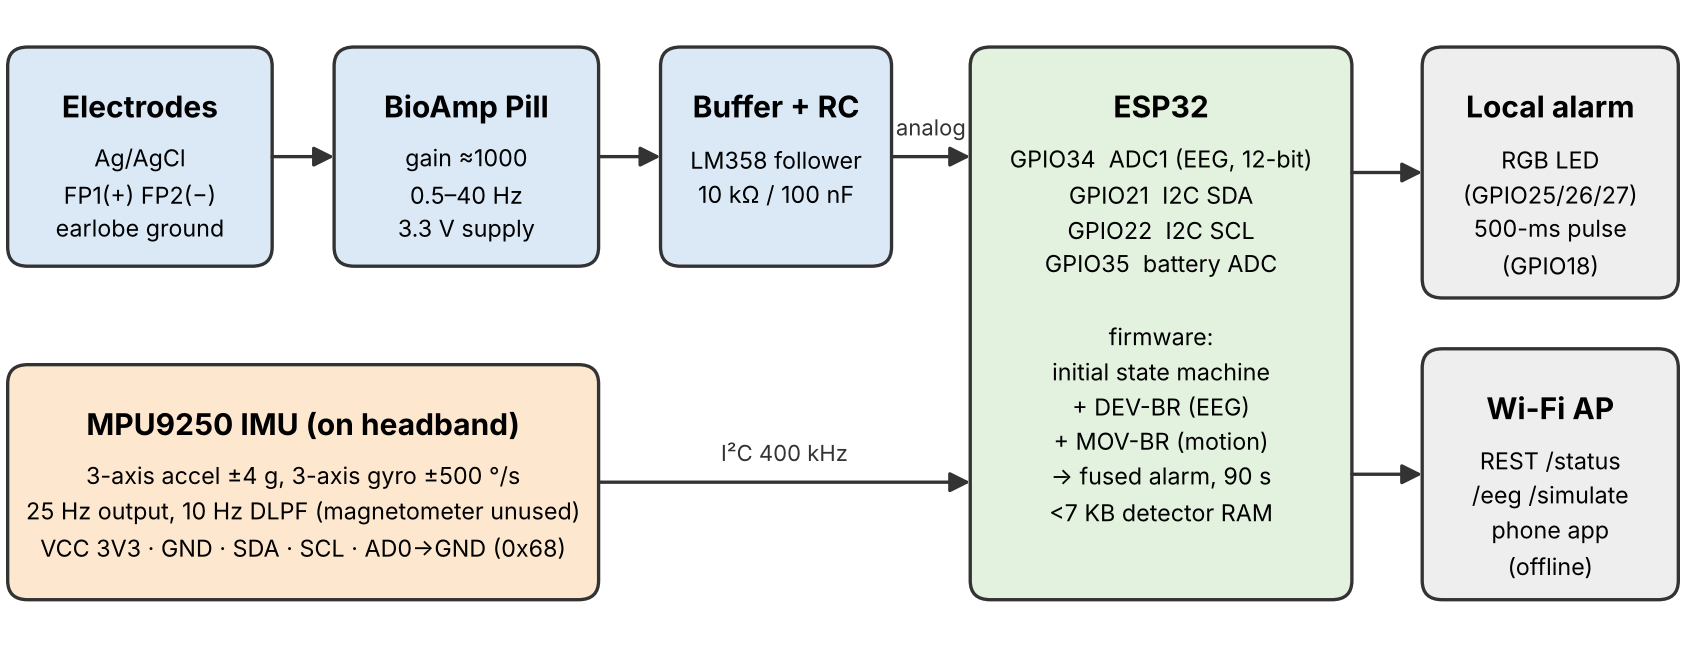
\includegraphics[width=0.86\textwidth]{figures/system.png}
\caption{Design. One forehead EEG channel (BioAmp Pill, LM358 follower, RC filter) feeds the ESP32 ADC; an MPU9250 on the headband is read over I$^2$C at 25~Hz. Gain and pass-band are nominal values from the documentation, not measurements.}
\label{fig:hw}
\end{figure*}

\begin{table}[t]
\centering
\caption{Implementation status and source of each specification.}
\label{tab:status}
\footnotesize
\setlength{\tabcolsep}{2pt}
\begin{tabular}{>{\raggedright\arraybackslash}p{0.17\columnwidth}>{\raggedright\arraybackslash}p{0.43\columnwidth}>{\raggedright\arraybackslash}p{0.34\columnwidth}}
\toprule
Item & Specification & Status / source \\
\midrule
EEG front-end & Ag/AgCl FP1$+$/FP2$-$; BioAmp Pill (gain $\approx$1000, 0.5--40~Hz, 3.3~V); LM358 follower; RC 159~Hz & prototype; nominal values, not measured here; vendor documents 5-V use~\cite{bioamp} \\
Motion sensor & MPU9250, $\pm$4~g, $\pm$500~$^\circ$/s, 10-Hz DLPF, 25~Hz, I$^2$C GPIO21/22~\cite{mpu9250} & implemented in firmware; no bench data \\
ADC, sampling & 12-bit, default attenuation, \texttt{delay(5)} loop & firmware reports measured rate \\
Outputs & RGB LED, 500-ms GPIO pulse, Wi-Fi AP REST API, phone app & firmware; app not evaluated \\
Detectors & EEG-only firmware: state machine + 3-feature analyzer; EEG-plus-motion firmware: DEV-BR, MOV-BR, joint alarm & EEG-only firmware replay-evaluated; EEG-plus-motion firmware compiled (792~KB flash), identical alarms offline \\
Bench / human data & noise, battery, timing, wear & not measured \\
\bottomrule
\end{tabular}
\end{table}

\textbf{Hardware.} One differential forehead channel is amplified by the BioAmp Pill, buffered by an LM358 and digitized by the ESP32; an MPU9250 accelerometer/gyroscope on the headband is read over I$^2$C (Fig.~\ref{fig:hw}, Table~\ref{tab:status}). The device runs from a USB battery bank without galvanic isolation. The LM358 is not rail-to-rail: at 3.3~V its output tops out near 1.8~V, about 150~mV above mid-supply~\cite{lm358}.

\textbf{Initial detectors.} The firmware tracks a baseline $b[n]{=}0.99\,b[n{-}1]{+}0.01\,x[n]$ and deviation $d[n]{=}|x[n]-\lfloor b[n]\rfloor|$, with an exponentially weighted mean $\mu$ and spread $\sigma$ (forgetting factor 0.995 per sample). Every 30~s it sets BROWNOUT and BLACKOUT thresholds to $\mu{+}2.5\sigma$ and $\mu{+}4\sigma$, clamped to fixed ADC ranges, and leaky counters confirm states. A Python analyzer computes line-length (LL), delta/alpha ratio and 30--45-Hz energy over 2.56~s and requires two of three features above adaptive thresholds on 7 of 8 ticks.

% =============================================================================
\section{Replay Evaluation}\label{sec:method}
\textbf{CHB-MIT}~\cite{shoeb2009thesis,goldberger2000physionet} has no FP1--FP2 channel. We derive it as the signed sum of seven bipolar channels, $(\text{FP1-F7})+(\text{F7-T7})+(\text{T7-FT9})+(\text{FT9-FT10})+(\text{FT10-T8})-(\text{F8-T8})-(\text{FP2-F8})$, which telescopes to FP1$-$FP2 \emph{if} all seven channels derive from one common reference with identical filtering; the dataset documentation does not confirm this and no measured FP1--FP2 exists to compare against. Consistency checks on \RcFiles{} recordings: calibration is identical across the chain, and eye-blink amplitude in the derived channel is \RcBlinkLo--\RcBlinkHi{} of that in FP1-F7 (common-mode ocular activity cancels), whereas a wrong-sign chain gives \RcWrongLo--\RcWrongHi; quantization noise of the sum is $\le$\RcQuantHi{}~$\mu$V rms. Three chb12 recordings are referential and use FP1$-$FP2 directly; five recordings without the chain were excluded. The analysis uses \NRec{} recordings (\NSz{} seizures, \NHours{}~h, \NSubj{} subjects; chb01 and chb21 are one subject): every seizure recording plus the first seizure-free recording of each patient, a subset of the archive, so FA/h describe these hours and not continuous wear. CHB-MIT has no motion data.
\textbf{SeizeIT2}~\cite{bhagubai2025seizeit2} (CC0) provides \SHours{}~h from \SNSubj{} patients with focal epilepsy recorded in five monitoring units with a wearable: two behind-the-ear EEG channels at 256~Hz and accelerometer/gyroscope data at 25~Hz from a sensor on the back of the neck, the head-borne location closest to our headband. It contains \SNSz{} annotated seizures (\SNFBTC{} focal-to-bilateral tonic--clonic, FBTC; \SNMotor{} focal motor; \SNNonMotor{} focal non-motor; \SNOther{} other). We use the single behind-the-ear channel of each recording (left or right side) as the device's EEG input; \SMovMissing{} of \SNRuns{} recordings lack head-motion data, and there motion detectors cannot fire.

\textbf{Front-end model and replay.} EEG passes a causal model of the nominal pass-band (0.5-Hz high-pass, 40-Hz low-pass), is resampled to 200~Hz, scaled by the nominal gain around 1.65~V and quantized to 12~bits. The analyzer is imported unmodified and driven by a simulated serial port and clock; the firmware \texttt{loop()} is ported line by line. Motion features are computed exactly as in the EEG-plus-motion firmware (Sec.~\ref{sec:det}). This is a software replay; no hardware-in-the-loop experiment was performed.

\textbf{Scoring.} Following SzCORE~\cite{dan2025szcore}, alarms within 90~s merge, a seizure counts as detected if an alarm falls in [onset$-$30~s, offset$+$60~s], and other alarms are false alarms (FA). Parameters are selected by leave-one-subject-out cross-validation (LOSO): on all other subjects we pick the most sensitive setting whose pooled FA/h meets a target and apply it to the held-out subject. CIs use a 2000-resample subject bootstrap; detectors are compared per subject with the Wilcoxon signed-rank test, and seizure-level detections with an exact McNemar test. Chance levels come from 200--1000 random circular shifts of each alarm train (restricted to the seizure class under test for convulsive results). Convulsive-mode comparisons use a sign test over patients, because seizures within a patient are correlated; CIs and parameter choices do not account for design decisions described below.

% =============================================================================
\section{Detectors}\label{sec:det}
\textbf{Why the initial detectors fail.} The firmware's spread estimate forgets within about 1~s, so 4$\sigma$ excursions are frequent in normal EEG; the analyzer's vote waits on two features that carry no seizure information (delta/alpha AUC \AucDAR{}, high-frequency energy \AucHFE{}); and fixed floors in ADC units make detection gain-dependent.

\textbf{DEV-BR and MOV-BR.} Let $\delta(t)$ be the per-second mean of the firmware deviation $d$, and $\alpha(t)$ the per-second mean of $\lVert \mathbf a - \mathrm{EMA}_{1\,\mathrm s}(\mathbf a)\rVert$ for the 25-Hz acceleration $\mathbf a$. For either signal $s$,
\begin{equation}
\rho_s(t) = \log \frac{s(t)}{\operatorname{median}\{s(\tau): t{-}329 \le \tau \le t{-}30\}},
\end{equation}
so each wearer is compared with their own background 30--330~s earlier and the units of the sensor cancel. A condition holds when $\rho \ge \log r$ for $D$ consecutive seconds; MOV-BR may also require that 2--7~Hz power (Hann window, last 4~s) exceed a share $q$, as in clonic jerking. The \emph{general mode} raises an event when the EEG \emph{or} the motion condition starts; the \emph{convulsive mode} raises an alarm when $\rho_\delta \ge \log r_E$ \emph{and} $\rho_\alpha \ge \log r_M$ hold together for $D$ seconds. Each output fires at most once per 90~s and not before 330~s. \emph{Design history:} the ratio rule, its window and lag, and the choice of the firmware deviation as the EEG signal were made after inspecting CHB-MIT results, and the convulsive mode, its parameter grid and the 0.02/0.05 FA/h targets were defined after the general mode failed to beat EEG alone (a first, narrower grid gave 64.5\% for FBTC seizures on all recordings). Leave-one-subject-out validation covers only the parameters, not these design choices, so the convulsive results are exploratory.

\textbf{EEG-plus-motion firmware.} The general event drives the BROWNOUT warning and the convulsive alarm drives BLACKOUT (red LED, GPIO pulse, app); the EEG-only firmware's serial format is unchanged. The detectors hold two 330-value histories and use \texttt{std::nth\_element} once per second (5~KB), plus 1.6~KB for motion features; it compiles for the ESP32 at 792~KB flash (EEG-only firmware: 767~KB). Its default parameters are the values most often selected by cross-validation: general mode $r{=}2$, $D{=}20$~s for EEG, $r{=}24$, $q{=}0.4$, $D{=}20$~s for motion (\SFusAParamsN{}/125 folds); convulsive mode $r_E{=}4$, $r_M{=}8$, $D{=}30$~s (\SCvAParamsN{}/125 folds of the all-recordings analysis; re-selection on the motion-equipped subset chose $r_E{=}6$, $r_M{=}3$ in \AvModalN{}/\AvSubjAll{} folds, and the firmware defaults give \AvDefDet{}/\AvDefN{} FBTC seizures at \AvDefFAday{} false alarms per day on that subset, in-sample and not held out). On the host, the C++ code matched the Python motion features to float precision and reproduced every alarm of the evaluation \SVerNote{}. It has not yet been timed on the ESP32.

% =============================================================================
\section{Results}\label{sec:res}
\begin{table*}[t]
\centering
\caption{CHB-MIT, FP1--FP2 (\NSubj{} subjects, \NSz{} seizures, \NHours{}~h; nominal front-end). Brackets: subject-bootstrap 95\% CI. ``Macro'': mean of per-subject sensitivities. ``Chance'': sensitivity of randomly circularly shifted alarms. BR rows: held-out subjects (LOSO).}
\label{tab:chb}
\begin{tabular}{lcccccc}
\toprule
Detector & Detected & Sensitivity [95\% CI] & Macro & FA/h & Latency (s) & Chance \\
\midrule
\MainTableBody
\bottomrule
\end{tabular}
\end{table*}

\begin{table*}[t]
\centering
\caption{SeizeIT2 (\SNSubj{} patients, \SNSz{} seizures, \SHours{}~h; behind-the-ear EEG through the device model, head-borne accelerometer). All non-firmware rows: held-out patients (LOSO). Class columns give the share of seizures of that class detected; ``Sleep'': seizures annotated as arising from sleep.}
\label{tab:s2}
\small
\setlength{\tabcolsep}{4pt}
\begin{tabular}{lcccccccc}
\toprule
Detector & Detected & Sensitivity [95\% CI] & FA/h & FBTC & Focal motor & Focal non-motor & Sleep & Chance \\
\midrule
\SMainTableBody
\bottomrule
\end{tabular}
\end{table*}

\begin{figure}[t]
\centering
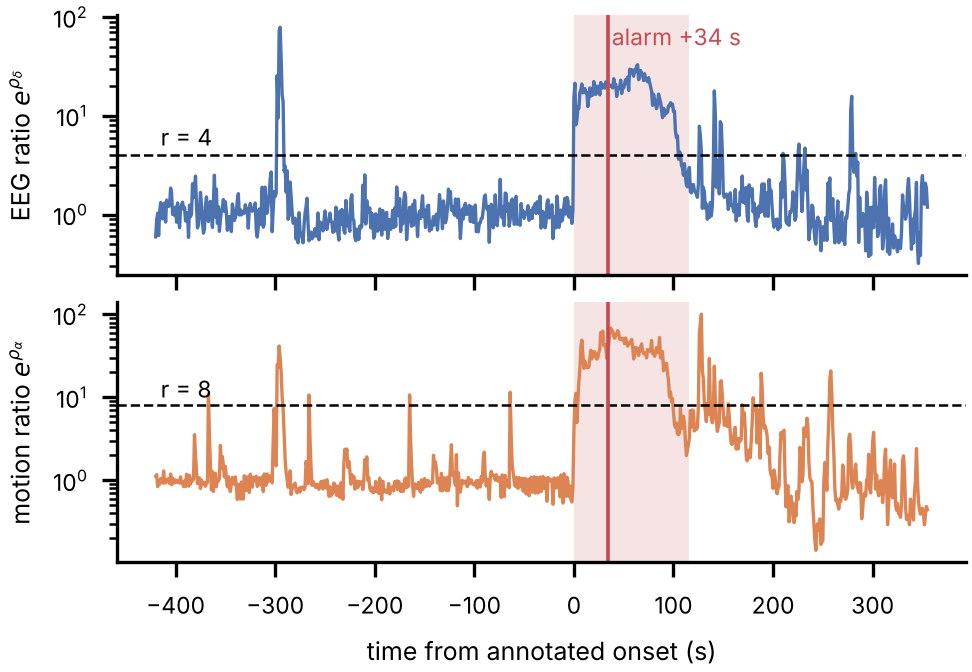
\includegraphics[width=0.95\columnwidth]{figures/convulsive_example.png}
\caption{Convulsive-mode alarm on an FBTC seizure (shaded) in SeizeIT2 patient 115, arising from sleep. Brief EEG artifacts and isolated movements cross one threshold but not both; the seizure raises both ratios and the alarm fires after the 30-s persistence. Shown: the detected sleep FBTC seizure with the shortest latency and no false alarm within 30~min (illustrative, not typical).}
\label{fig:example}
\end{figure}

\begin{table}[t]
\centering
\caption{CHB-MIT front-end robustness (simulated). ``Fixed'': DEV-BR with $r{=}\HwFixR$, $D{=}\HwFixD$~s chosen at gain 1000. Clip: LM358 1.8-V ceiling; Sat.: saturated samples. Cells: sensitivity / FA/h.}
\label{tab:hw}
\footnotesize
\setlength{\tabcolsep}{1.5pt}
\begin{tabular}{lcccc}
\toprule
Condition & Sat. & DEV-BR fixed & DEV-BR LOSO & Firmware \\
\midrule
\HwTableBody
\bottomrule
\end{tabular}
\end{table}

\begin{figure}[t]
\centering
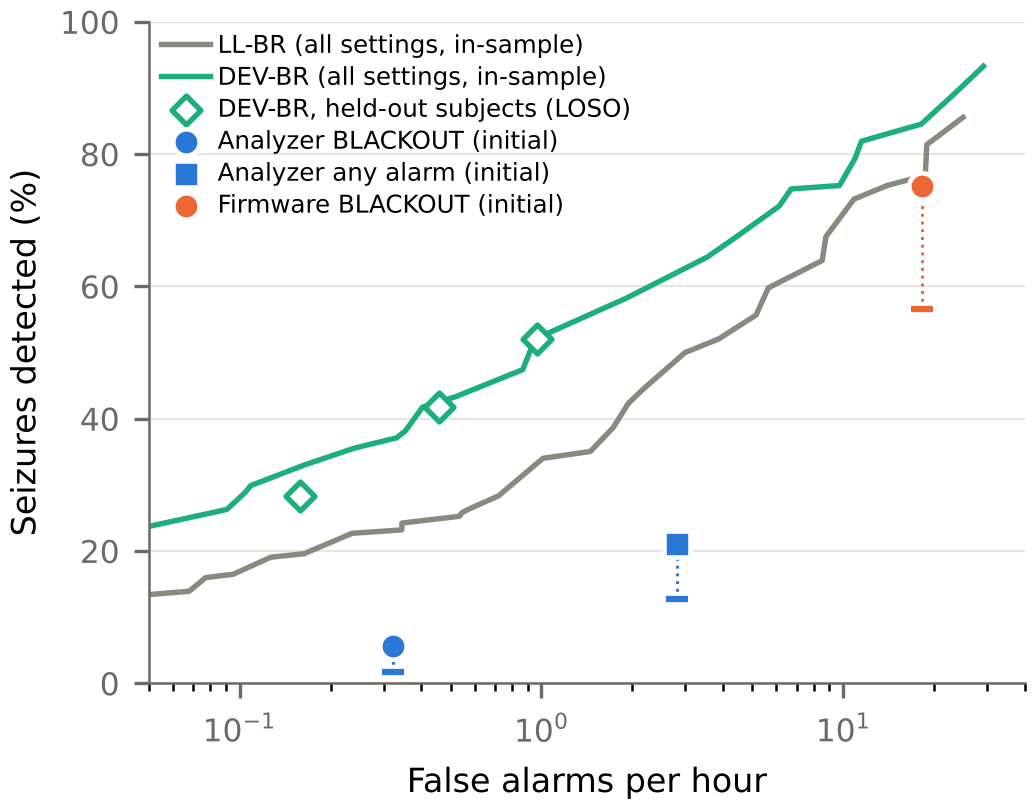
\includegraphics[width=0.88\columnwidth]{figures/operating_curve.png}
\caption{CHB-MIT, FP1--FP2: sensitivity versus FA/h. Lines: best in-sample ratio trade-offs; diamonds: DEV-BR on held-out subjects; markers: initial detectors, with dashes at their chance levels.}
\label{fig:roc}
\end{figure}

\textbf{CHB-MIT (reconstructed FP1--FP2, EEG only).} The analyzer's BLACKOUT alarm detected \PyBSens{} at \PyBFAh{}~FA/h; the firmware reached \FwBSens{} at \FwBFAh{}~FA/h, but randomly shifted copies of its alarms already reach \FwBNull{} (Table~\ref{tab:chb}). DEV-BR detected \DevADet{}/\NSz{} seizures (\DevASens{}, CI \DevACI{}) at \DevAFAh{}~FA/h with a median latency of \DevALat{}~s (Fig.~\ref{fig:roc}), against a chance level of \DevANull{}. At a lower alarm rate, \DevBSens{} at \DevBFAh{}~FA/h, it detected about \FoldDevPy{} times as many seizures as the analyzer (\PyBSens{} at \PyBFAh{}~FA/h) and was better in \TestDevPyBetter{} of \TestDevPyN{} subjects and worse in none (\TestDevPyP{}); the operating points differ, so this comparison is indicative. Without normalization the same procedure reached \AblAbsSens{}, and logistic regression and boosted trees on 14 normalized features did not do better (best \AltBestOneSens{} at $\le$1~FA/h). In simulation, with parameters frozen, DEV-BR stayed at \HwDevSensMin{}--\HwDevSensMax{} and \HwDevFAMin{}--\HwDevFAMax{}~FA/h across modelled gains of 500--2000, LM358 clipping, a 3.1-V ADC range and a 6-ms loop, while the firmware moved between \HwFwSensMin{} and \HwFwSensMax{} at \HwFwFAMin{}--\HwFwFAMax{}~FA/h (Table~\ref{tab:hw}). These are software simulations of assumed errors; no hardware was varied or measured.

\begin{figure*}[t]
\centering
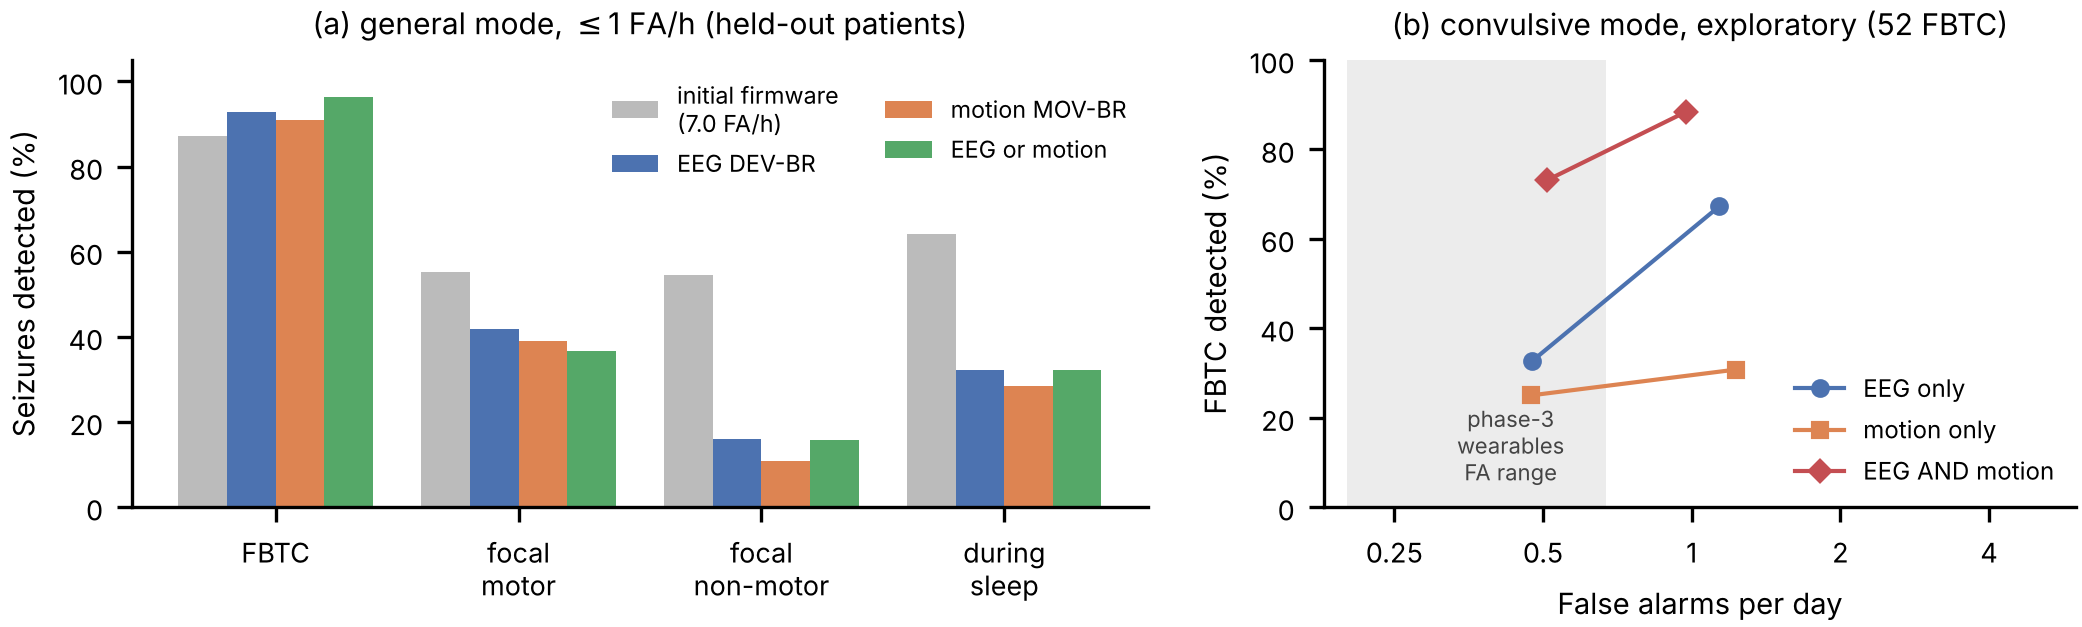
\includegraphics[width=0.92\textwidth]{figures/seizeit2_results.png}
\caption{SeizeIT2, held-out patients. (a) Share of seizures detected by class at $\le$1~FA/h (the initial firmware at its own 7.0~FA/h). (b) Convulsive mode (exploratory; recordings with a motion channel): FBTC sensitivity versus false alarms per day for LOSO targets of 0.02 and 0.05~FA/h; shaded, the false-alarm range reported for phase-3 wearables~\cite{beniczky2021guideline}, which were tested on different data.}
\label{fig:s2}
\end{figure*}

\textbf{SeizeIT2: initial firmware and general mode.} On behind-the-ear EEG the initial firmware detected \SFwSens{} at \SFwFAh{}~FA/h (\SFwFAday{} per day), against a chance level of \SFwNull{} (Table~\ref{tab:s2}). At the same alarm rate, EEG-or-motion detected \SFusFwSens{} (\STFUSEDFwVFWBetter{} patients better, \STFUSEDFwVFWWorse{} worse, \STFUSEDFwVFWP{}) and DEV-BR alone \SEegFwSens{}. At $\le$1~FA/h, DEV-BR detected \SEegASens{} (macro \SEegAMacro{}; chance \SEegANull{}), MOV-BR \SMovASens{}, and their combination \SFusASens{}: motion detected seizures the EEG missed but added as many false alarms, so the general mode did not beat EEG alone (\STFUSEDAVEEGAP{}). Gyroscope magnitude was weaker than acceleration (\SGyrASens{}), and a rhythm gate was selected in every MOV-BR fold. Detection depended strongly on seizure type (Fig.~\ref{fig:s2}a); the high FBTC share below comes at about 23 false alarms per day: \SFusAFBTC{} of FBTC seizures, \SFusAMot{} of focal motor and \SFusANonMot{} of focal non-motor seizures.

\textbf{SeizeIT2: convulsive mode (exploratory).} This mode needs a motion channel, so it is evaluated on the \AvRuns{} recordings that have one (\AvHours{}~h; \AvFbtc{} FBTC seizures in \AvSubj{} patients; Table~\ref{tab:cv}). With parameters chosen for FBTC seizures at $\le$0.02~FA/h, requiring EEG and head motion to rise together detected \AvCoADet{}/\AvCoAN{} FBTC seizures (\AvCoASens{}, CI \AvCoACI{}) at \AvCoAFAday{} false alarms per day, against a class-specific chance level of \AvCoANull{} (\AvCoAPNull{}). EEG alone detected \AvEgASens{} and motion alone \AvMvASens{} at the same rate. Per patient, the joint alarm was better than EEG alone in \AvEegABetter{} patients and worse in \AvEegAWorse{} (\AvEegAP{}, sign test; \AvEegATied{} tied) and better than motion alone in \AvMovABetter{} and worse in \AvMovAWorse{} (\AvMovAP{}). The median latency was \AvLat{}~s (IQR \AvLatIQR{}) from the annotated focal onset, which precedes bilateral spread; \AvSleepDet{} of \AvSleepN{} seizures arising from sleep were detected, and \AvZeroFA{} of \AvSubjAll{} patients had no false alarm. With a 0.05-FA/h target the joint alarm detected \AvCoBDet{}/\AvCoBN{} (\AvCoBSens{}, CI \AvCoBCI{}) at \AvCoBFAday{} false alarms per day (Fig.~\ref{fig:s2}b). Because the 95\% CIs reflect patient sampling only and not the design choices above, they are optimistic.

\begin{table}[t]
\centering
\caption{SeizeIT2 convulsive mode, restricted to recordings with a motion channel (\AvRuns{} recordings, \AvFbtc{} FBTC seizures, \AvSubj{} patients; held-out patients, exploratory). Chance: mean FBTC sensitivity of randomly circularly shifted alarm trains (95th percentile $\le$\AvCoANullP{} for all rows shown).}
\label{tab:cv}
\scriptsize
\setlength{\tabcolsep}{2pt}
\begin{tabular}{llccc}
\toprule
Target & Detector & FBTC detected [95\% CI] & FA/day & Chance \\
\midrule
$\le$0.02 FA/h & EEG only & \AvEgADet/\AvEgAN{} ({\AvEgASens}) [\AvEgACI] & \AvEgAFAday & \AvEgANull \\
 & Motion only & \AvMvADet/\AvMvAN{} ({\AvMvASens}) [\AvMvACI] & \AvMvAFAday & \AvMvANull \\
 & \textbf{EEG AND motion} & \AvCoADet/\AvCoAN{} ({\AvCoASens}) [\AvCoACI] & \AvCoAFAday & \AvCoANull \\
$\le$0.05 FA/h & EEG only & \AvEgBDet/\AvEgBN{} ({\AvEgBSens}) [\AvEgBCI] & \AvEgBFAday & \AvEgBNull \\
 & Motion only & \AvMvBDet/\AvMvBN{} ({\AvMvBSens}) [\AvMvBCI] & \AvMvBFAday & \AvMvBNull \\
 & \textbf{EEG AND motion} & \AvCoBDet/\AvCoBN{} ({\AvCoBSens}) [\AvCoBCI] & \AvCoBFAday & \AvCoBNull \\
\bottomrule
\end{tabular}
\end{table}

% =============================================================================
\section{Discussion and Limitations}
Replaying the firmware code showed that the EEG-only prototype's alarms mostly fire at random, and that one rule, comparing a signal with the wearer's own delayed median, improves EEG detection and transfers to a motion sensor without knowing its units. In this software replay, adding head motion improved detection of convulsive seizures: neither modality alone reached a low false-alarm rate at 0.5 alarms per day, but the joint alarm detected about three in four FBTC seizures at a false-alarm rate comparable to that reported for phase-3 wearables, with under 7~KB of RAM and no machine learning. This comparison is indirect (different data and populations) and exploratory. The results suggest three practices: test the firmware code itself rather than a re-implementation; normalize each signal against the wearer's own background so decisions do not depend on sensor units or gain; and require both modalities to agree when the target event changes both.

The absolute performance still falls short. Clinical wearables reach 90--96\% for tonic--clonic seizures~\cite{beniczky2021guideline}, and a learned EEG-plus-EMG model on a SeizeIT2 subset reached 97.7\% at 0.4 false positives per 24~h~\cite{zhang2024multimodal}; focal non-motor seizures were rarely detected at 1~FA/h or fewer. Limitations: (i)~all results come from software replay; no recordings from the prototype, bench measurements of the MPU9250 or front-end, or human tests are reported. (ii)~SeizeIT2 differs from the device: its EEG is behind-the-ear rather than FP1--FP2, its motion sensor sits on the neck at 25~Hz rather than on the headband, and it was recorded in hospital. (iii)~The front-end model uses nominal values; non-idealities were simulated, not measured, and the BioAmp runs below its documented supply. (iv)~FBTC results rest on \AvCoAN{} seizures from \AvSubj{} patients and an exploratory design. (v)~the firmware defaults are the values most often selected by cross-validation on the same data, and the firmware has not been timed on the ESP32. (vi)~FP1--FP2 on CHB-MIT is derived, not measured, and FA/h come from a subset of recordings. Next steps are bench characterization, overnight recordings, and an ethics-approved study.

% =============================================================================
\section{Conclusion}
We developed a low-cost EEG and head-motion epilepsy seizure alarm and evaluated its code as written, by software replay, on two public datasets (\NSubj{} and \SNSubj{} patients). The initial detectors fail for identifiable reasons. A delayed-median ratio rule improves the EEG detector (\DevASens{} at \DevAFAh{}~FA/h on reconstructed FP1--FP2, stable in simulated front-end errors), and in an exploratory analysis requiring EEG and motion to agree detected \AvCoASens{} of FBTC seizures at \AvCoAFAday{} false alarms per day, in firmware that fits in under 7~KB of RAM. Confirming these results requires bench measurements and recordings from people. Firmware, analyzer, replay code and detectors are provided for others to reproduce and extend.

\section*{Data and Code Availability}
CHB-MIT~\cite{goldberger2000physionet} and SeizeIT2~\cite{bhagubai2025seizeit2} are public. Firmware (EEG-only and EEG-plus-motion), analyzer, schematics, replay code, the C++ detectors and the audit scripts are at~\cite{vera_repo}.

\bibliographystyle{IEEEtran}
\bibliography{refs}

\end{document}
